\section{Introduction}
\begin{frame}{$\mathbf{\theta}$-Curves}
	\begin{itemize}
		\item A \term{$\theta$-curve} $T$ is a graph embedded in $S^3$,
		which consists of two vertices $v_1$, $v_2$
		and three edges $e_1$, $e_2$, $e_3$,
		such that each edge joins the vertices.
		\item A \term{constituent knot $T_{ij}$}, $1 \le i < j \le 3$, is a subgraph of $T$
		that consists of two vertices $v_1$, $v_2$ and two edges $e_i$, $e_j$.
		
		\item $\theta$-curves are roughly classified by comparing the triples of constituent knots.
		
		\item A $\theta$-curve is said to be \term{trivial} if it can be embedded in a 2-sphere in $S^3$.

		$$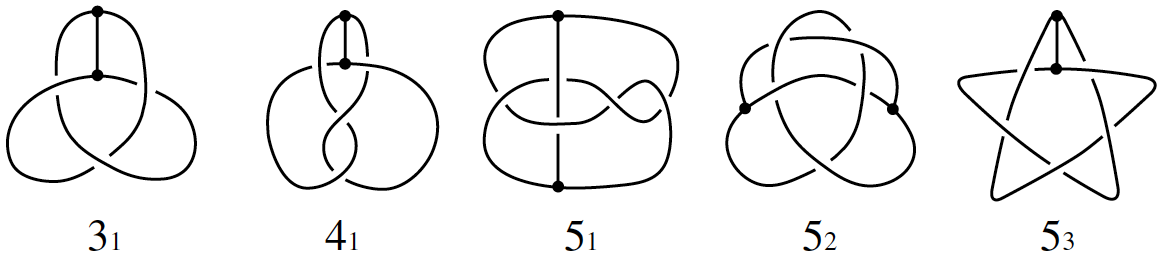
\includegraphics[width=.8\linewidth]{theta_exe.png}$$
	\end{itemize}
	
	\seprule
	\hfill\tiny{Figure from \cite{theta_7}}
\end{frame}

\begin{frame}{Handcuff-Graphs}
	\begin{itemize}
		\item \term{Handcuff graph} consists of $2$ loops and $1$ edge joining the loops.
	\end{itemize}

	$$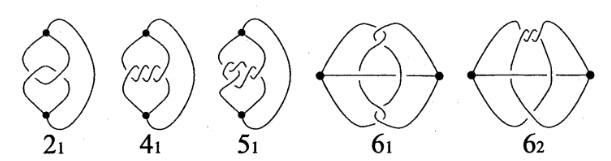
\includegraphics[width=.8\linewidth]{handcufflist.png}$$
	\seprule
	\hfill\tiny{Figure from \cite{handcufflist}}
	% 모리우치 A table of 0-curves and handcuff graphs
with up to seven crossings
\end{frame}

\begin{frame}{Reidemaister Moves for $\theta$-Curves}
	\medskip
	\begin{enumerate}
		\item[\mybf{I.}] \quad\raisebox{-15pt}{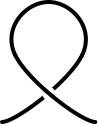
\includegraphics[width=36pt,height=36pt]{y101}} \quad $\longleftrightarrow$ \quad \raisebox{-15pt}{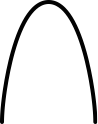
\includegraphics[width=36pt,height=36pt]{y103}} \quad $\longleftrightarrow$ \quad \raisebox{-15pt}{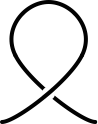
\includegraphics[width=36pt,height=36pt]{y102}}\medskip
		\item[\mybf{II.}] \quad\raisebox{-15pt}{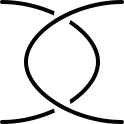
\includegraphics[width=36pt,height=36pt]{y111}} \quad $\longleftrightarrow$ \quad \raisebox{-15pt}{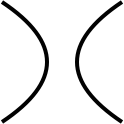
\includegraphics[width=36pt,height=36pt]{y93}} \quad $\longleftrightarrow$ \quad \raisebox{-15pt}{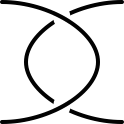
\includegraphics[width=36pt,height=36pt]{y112}}\medskip
		\item[\mybf{III.}] \quad\raisebox{-15pt}{
\includegraphics[width=36pt,height=36pt]{r31}} \quad $\longleftrightarrow$ \quad \raisebox{-15pt}{
\includegraphics[width=36pt,height=36pt]{r32}} \qquad\qquad\raisebox{-15pt}{
\includegraphics[width=36pt,height=36pt]{y121}} \quad $\longleftrightarrow$ \quad \raisebox{-15pt}{
\includegraphics[width=36pt,height=36pt]{y122}}\medskip
		\item[\mybf{IV.}] \quad\raisebox{-15pt}{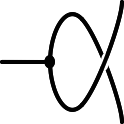
\includegraphics[width=36pt,height=36pt]{y141}} \quad $\longleftrightarrow$ \quad \raisebox{-15pt}{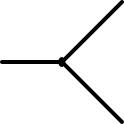
\includegraphics[width=36pt,height=36pt]{y143}} \quad $\longleftrightarrow$ \quad \raisebox{-15pt}{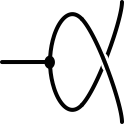
\includegraphics[width=36pt,height=36pt]{y142}}\medskip
		\item[\mybf{V.}] \quad\raisebox{-15pt}{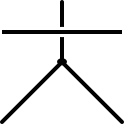
\includegraphics[width=36pt,height=36pt]{y131}} \quad $\longleftrightarrow$ \quad \raisebox{-15pt}{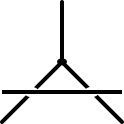
\includegraphics[width=36pt,height=36pt]{y132}} \qquad\qquad\raisebox{-15pt}{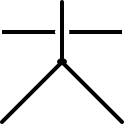
\includegraphics[width=36pt,height=36pt]{y133}} \quad $\longleftrightarrow$ \quad \raisebox{-15pt}{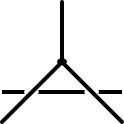
\includegraphics[width=36pt,height=36pt]{y134}}
	\end{enumerate}
\end{frame}


\begin{frame}{Arc Index}
	\begin{itemize}
		\item An \term{arc presentation} of a $\theta$-curve is defined in the same
		manner as an arc presentation of a knot.
		
		\item The binding axis contains all \term{vertices} of $\theta$-curve.

		\item \term{Minimal arc presentation} and \term{arc index} are defined in the same manner.		
	\end{itemize}
	\begin{tabu}{X[c]X[c]X[c]X[c]}
		\raisebox{-1cm}{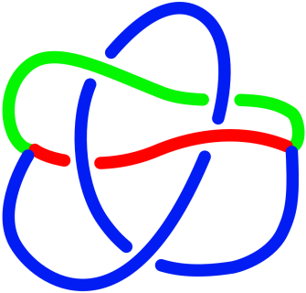
\includegraphics[height=2cm]{theta52.png}} &
		\raisebox{-1.8cm}{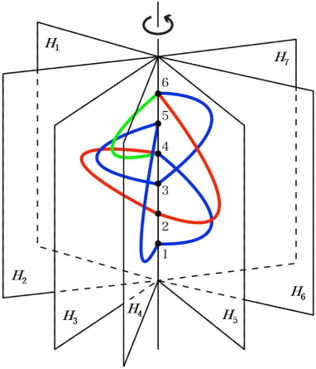
\includegraphics[height=3.6cm]{openbook.png}} &
		\raisebox{-1cm}{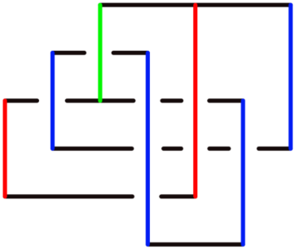
\includegraphics[height=2cm]{grid.png}} &
		\raisebox{-1.8cm}{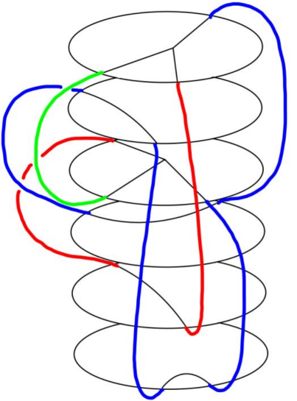
\includegraphics[height=3.6cm]{stacked.png}}\\
		% & & & \\
		$\theta5_2$ & Open Book & Grid Diagram & Stacked Tangle 
		\end{tabu}
		
\end{frame}

\begin{frame}{Grid Diagram}
	\begin{itemize}
		\item The \term{grid diagram} is a handcuff graph or theta‐curve diagram of vertical strands and one less number of horizontal strands with the properties that at every crossing the vertical strand crosses over the horizontal strand and no two horizontal segments are co‐linear and no two vertical segments are co‐linear.
		\item If the number of half planes in arc presentation is $\alpha$, then the size of corresponding grid diagram is $(\alpha - 1) \s \alpha$.
	\end{itemize}
\begin{figure}
    \centerline{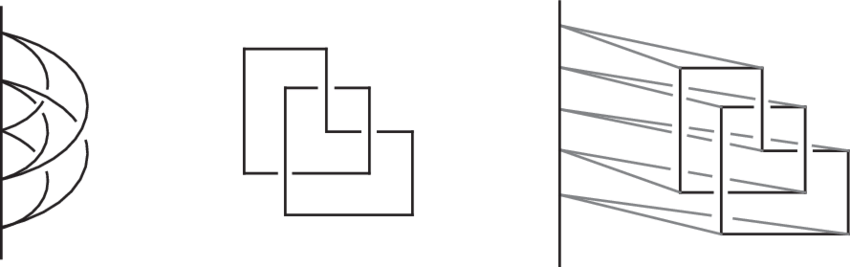
\includegraphics[width=0.5\linewidth]{../figs/An_arc_presentation_and_a_grid_diagram_of_the_knot.png}}
\end{figure}
\end{frame}

% \begin{frame}{Binding Circle Method}
% 	Let $D_T$ be a diagram of an $\theta$-curve $T$.
% 	A \term{binding circle} of $D_T$ is a simple closed curve $C$ meeting $D_T$
% 	in $n$ distinct points with the following properties:
% 	\begin{columns}
% 		\begin{column}{.7\textwidth}
% 			\begin{itemize}
% 				\item $C$ must meet $D_T$ at \term{two vertices}.
% 				\item $C$ divide $D_T$ into $n$ arcs $\alpha_1$, $\alpha_2$, $\ldots$, $\alpha_n$.
% 				\item Each $\alpha_i$ has no self-crossings.
% 				\item If $\alpha_i$ crosses over $\alpha_j$ at a crossing in inside(resp. outside) $C$,
% 				then $i < j$(resp. $i > j$) and it crosses over $\alpha_i$ at any other crossings with $\alpha_j$, respectively.
% 				\item For each $i$, there exists an embedded disk $d_i$ such that $\partial d_i = C$ and $\alpha_i \subset d_i$.
% 				\item $d_i \cap d_j = C$, for distinct $i$ and $j$.
% 			\end{itemize}
% 		\end{column}

% 		\begin{column}{.3\textwidth}
% 			$$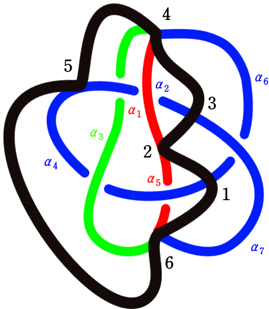
\includegraphics[width=.95\linewidth]{algorithm_binding.png}$$			
% 		\end{column}
% 	\end{columns}
% 	Then the pair $(D_T, C)$ is also corresponding to an arc presentation.
% \end{frame}


\begin{frame}{Binding Circle Method}
	\begin{tabu}{X[5c]X[c]X[5c]X[c]X[5c]}
		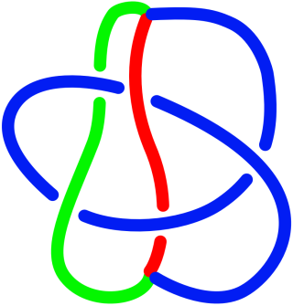
\includegraphics[width=.95\linewidth]{theta52c.png} & \raisebox{1.5cm}{$\longrightarrow$} & 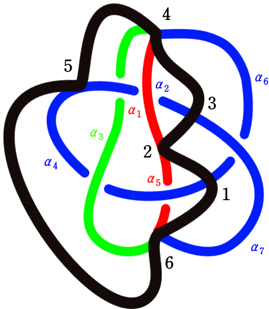
\includegraphics[width=.95\linewidth]{algorithm_binding.png} & \raisebox{1.5cm}{$\longleftrightarrow$} & 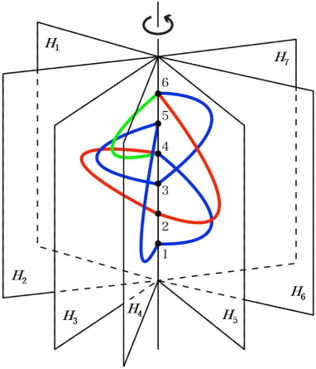
\includegraphics[width=.95\linewidth]{openbook.png}
	\end{tabu}
\end{frame}


\begin{frame}{Upper Bound of Arc Index}

	\begin{thm}[\cite{arc_spacial}]
		Let $G$ be any spatial graph with $e$ edges and $b$ bouquet cut components.
		Then
		\[
			\alpha(G) \le c(G) + e + b
		\]
	\end{thm}

	\begin{cor}
		Let $T$ be any $\theta$-curve.
		Then
		\[
			\alpha(T) \le c(T) + 3
		\]
	\end{cor}
\end{frame}
\section{Classifying by Determinant}
\begin{frame}{Determinant of the cromwell matrices of Knot}
	\begin{thm}
		Let $K$ be any knot then its determinant of the cromwell matrix is $0$ or $2$.
	\end{thm}
\end{frame}

\section{Lower Bounds of Arc Index}

\begin{frame}{Lower Bounds from Constituent Knots}
	\begin{thm}
		Let $T$ be any $\theta$-curve
		and $K_1$, $K_2$, $K_3$ be three constituent knots of $T$.
		Then
		\[
			\alpha(T) \ge \max_{i\in\{1,2,3\}} \alpha(K_i) + 1
		\]
	\end{thm}

	\mypf

	\begin{tabu}{X[c]X[c]X[c]X[c]}
			\raisebox{-1.5cm}{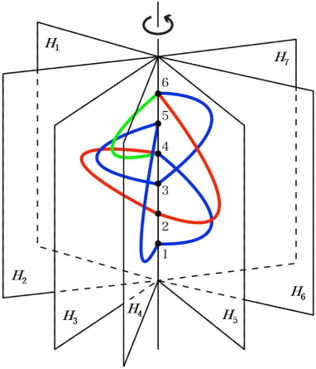
\includegraphics[height=3cm]{openbook.png}} &
			\raisebox{-1.5cm}{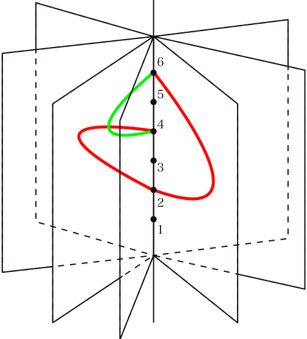
\includegraphics[height=3cm]{openbook_k1.png}} &
			\raisebox{-1.5cm}{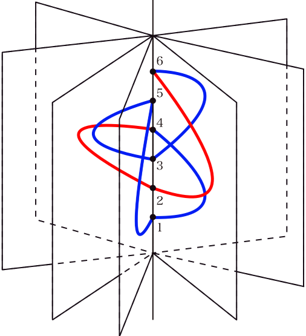
\includegraphics[height=3cm]{openbook_k2.png}} &
			\raisebox{-1.5cm}{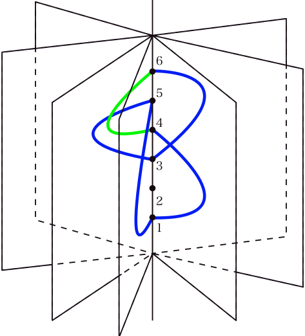
\includegraphics[height=3cm]{openbook_k3.png}}
	\end{tabu}
	\hfill\qed
\end{frame}


\begin{frame}
	\bigskip
	\begin{thm}
		Let $T$ be any $\theta$-curve
		and $K_1$, $K_2$, $K_3$ be three constituent knots of $T$.
		Then
		\[
			\centerline{$\displaystyle\alpha(T) \ge \frac12 \sum_{i=1}^3\alpha(K_i)$}
		\]
	\end{thm}
	
	\mypf

	\begin{itemize}
		\item A minimal arc presentation of $T$ is given.
		\item $K_1 = e_1\cup e_2$, $K_2 = e_2\cup e_3$, and $K_3 = e_3\cup e_1$.
		\item $S_i$ be the set of half plane corresponding the edge $e_i$.
		\item $S_i\cup S_{i+1}$ form an arc presentation of the knot $K_i$.
		\item $\alpha(K_i) \le |S_i| + |S_{i+1}|$
	\end{itemize}
	\[
		\sum_{i=1}^3 \alpha(K_i) \le 2\sum_{i=1}^3|S_i| = 2 \alpha(T)
	\]
	\hfill\qed
\end{frame}


\begin{frame}{Stacked Tangle of an $\theta$-Curve}
	\begin{tabu}{X[c,8]X[c,8]X[c,10]X[c,10]}
		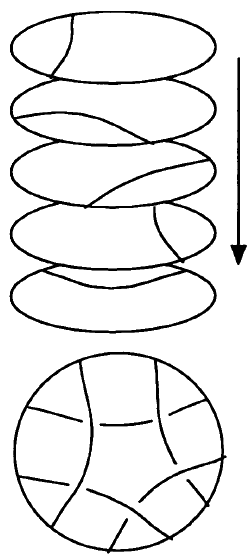
\includegraphics[width=\linewidth]{stacked_tangle.png} & 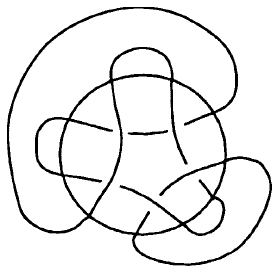
\includegraphics[width=\linewidth]{stacked_tangle2.png} & 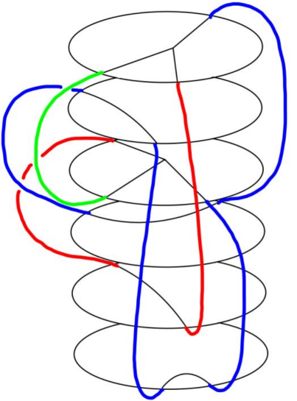
\includegraphics[width=\linewidth]{stacked.png} & 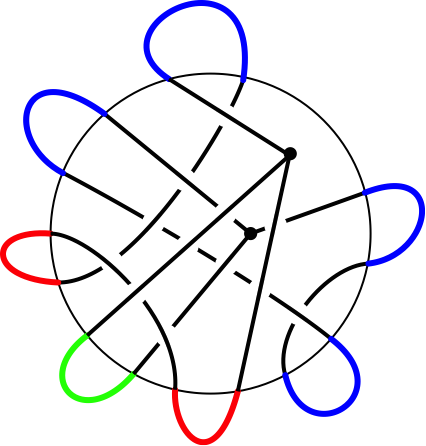
\includegraphics[width=\linewidth]{stacked_theta.png}\\
		\multicolumn{2}{c}{Stacked Tangle of a Link} & \multicolumn{2}{c}{Stacked Tangle of a $\theta$-Curve}
	\end{tabu}
	\seprule
	\tiny{Figure from \cite{arc_kauffman}}
\end{frame}


\begin{frame}
	\term{Stacked tangle} of an $\theta$-curve is stacked disks each with the frame as boundary with following properties:
	\begin{columns}
		\begin{column}{0.8\textwidth}
			\begin{itemize}
				\item Only two disk called \term{non-simple disks} contain one vertex and three line segments which joins the vertex and boundary point.
				\item One of the non-simple discs is at the top.
				\item Other disks called \term{simple disks} contain simple arc which joins two points on the boundary.
				\item When view from above
				\begin{itemize}
					\item two arcs in different simple disks intersect at most one point(by RII)
					\item arc in simple disk and tree in non-simple disk intersect at most one point(by RV)
				\end{itemize}
			\end{itemize}
		\end{column}

		\begin{column}{0.2\textwidth}
			$$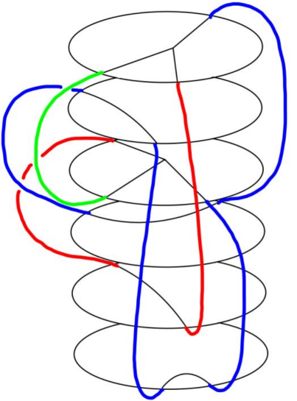
\includegraphics[width=\linewidth]{stacked.png}$$
		\end{column}
	\end{columns}
\end{frame}


\begin{frame}
	\term{Simple closure} of stacked tangle is a \term{stacked tangle} with \term{caps} satisfying following properties:
	\vspace*{-10pt}
	\begin{columns}
		\begin{column}{.8\textwidth}
			\begin{itemize}
				\item A \term{cap} is a simple arc in outside of stacked tangle joining end points of arcs or line segments.
				\item When view from above any tow caps have no intersection.
			\end{itemize}					
			Then a simple closure of a stacked tangle \myem{without any nested caps} is corresponding to an arc presentation.
		\end{column}

	\begin{column}{.2\textwidth}
		$$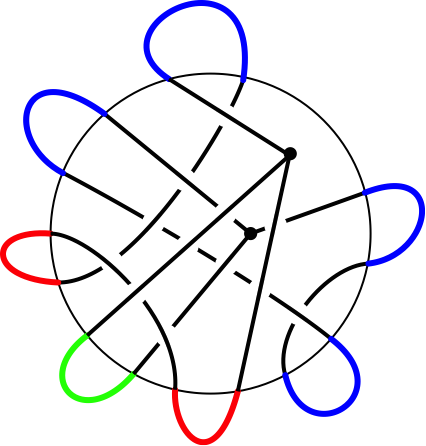
\includegraphics[width=\linewidth]{stacked_theta.png}$$
	\end{column}
	\end{columns}
	A \term{reduced simple closure of a stacked tangle} is 
	\begin{itemize}
		\item a simple closure of a stacked tangle \myem{without any nested caps}
		\item any two arcs(including line segment) joining by caps have \myem{no intersection} when view from above
	\end{itemize}
\end{frame}


\begin{frame}
	\begin{prop}
		A reduced simple closure of a stacked tangle
		can be obtained a simple closure of a stacked tangle without any nested caps by applying Reidemaister Moves.
	\end{prop}
	\mypf
	\vspace*{-12pt}
	$$\raisebox{-.13\textheight}{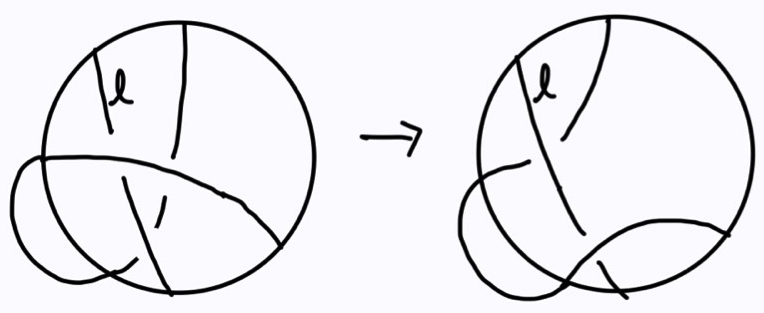
\includegraphics[height=.26\textheight]{reduced_stacked1.png}}\qquad\raisebox{-.3\textheight}{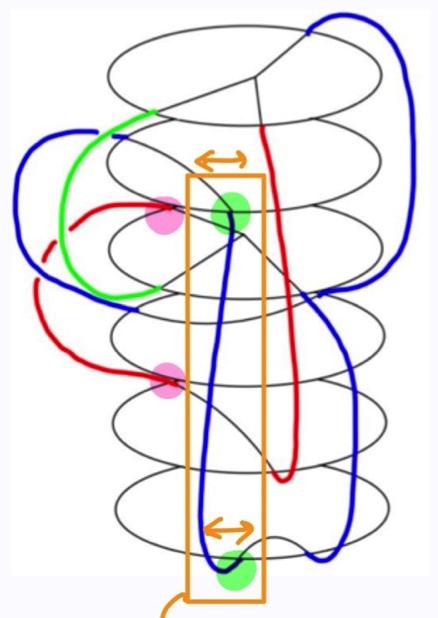
\includegraphics[height=.6\textheight]{reduced_stacked2.png}}\qquad\raisebox{-.2\textheight}{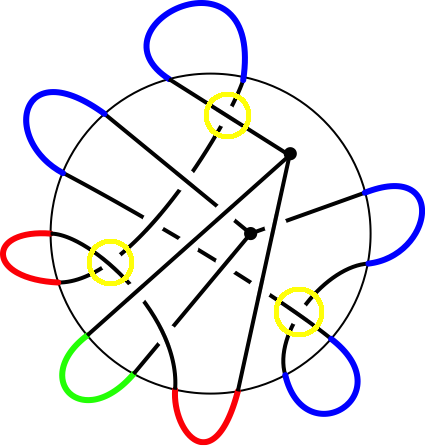
\includegraphics[height=.4\textheight]{reduced_stacked3.png}}$$
	\hfill\qed
\end{frame}


\begin{frame}{Yamada Polynomials}
	Let $D_T$ be a diagram of an $\theta$-curve $T$.
	Then, the \term{Yamada Polynomial $R(D_T)\in \mathbf{Z}\left[x^{\pm1}\right]$} is calculated by the following properties:
	\begin{itemize}
		\item \myem{Y6:} $R\left(\raisebox{-3pt}{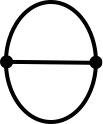
\includegraphics[height=12pt]{y6}}\right)= - (x+1+x^{-1})(x + x^{-1}) = -x^2 - x - 2 - x^{-1} - x^{-2}$\hfill \myem{Y7:} $R\left(\raisebox{-1.5pt}{
\includegraphics[height=8pt]{y7}}\right)=0$
		\item \myem{Y8:} $R(T'\cup\bigcirc) = (x+1+x^{-1})R(T')$ for an arbitrary $\theta$-curve diagram $T'$
		\item \myem{Y9:} $R\left(\raisebox{-3pt}{
\includegraphics[height=12pt]{y91}}\right)-R\left(\raisebox{-3pt}{
\includegraphics[height=12pt]{y92}}\right)=(x-x^{-1})\left[R\left(\raisebox{-3pt}{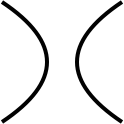
\includegraphics[height=12pt]{y93}}\right)-R\left(\raisebox{-3pt}{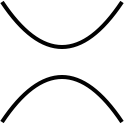
\includegraphics[height=12pt]{y94}}\right)\right]$
		\item \myem{Y10:} $R\left(\raisebox{-3pt}{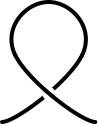
\includegraphics[height=12pt]{y101}}\right) = x^2 R\left(\raisebox{-3pt}{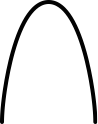
\includegraphics[height=12pt]{y103}}\right)$,\quad
		$R\left(\raisebox{-3pt}{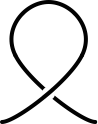
\includegraphics[height=12pt]{y102}}\right) = x^{-2} R\left(\raisebox{-3pt}{\includegraphics[height=12pt]{y103}}\right)$
		\item \myem{Y11:} $R\left(\raisebox{-3pt}{\includegraphics[height=12pt]{y111}}\right) = R\left(\raisebox{-3pt}{\includegraphics[height=12pt]{y93}}\right)$\hfill
		\myem{Y12:} $R\left(\raisebox{-3pt}{\includegraphics[height=12pt]{y121}}\right) = R\left(\raisebox{-3pt}{\includegraphics[height=12pt]{y122}}\right)$
		\item \myem{Y13:} $R\left(\raisebox{-3pt}{\includegraphics[height=12pt]{y131}}\right) = R\left(\raisebox{-3pt}{\includegraphics[height=12pt]{y132}}\right)$,\quad $R\left(\raisebox{-3pt}{\includegraphics[height=12pt]{y133}}\right) = R\left(\raisebox{-3pt}{\includegraphics[height=12pt]{y134}}\right)$
		\item \myem{Y14:} $R\left(\raisebox{-3pt}{\includegraphics[height=12pt]{y141}}\right) = -x R\left(\raisebox{-3pt}{\includegraphics[height=12pt]{y143}}\right)$,\quad $R\left(\raisebox{-3pt}{\includegraphics[height=12pt]{y142}}\right) = -x^{-1}R\left(\raisebox{-3pt}{\includegraphics[height=12pt]{y143}}\right)$
	\end{itemize}

	\begin{prop}[\cite{yamada}]
		$R(D_T)$ is an ambient isotopy invariant of $T$ up to multiplying $(-x)^n$ for some integer $n$.
	\end{prop}
\end{frame}


\begin{frame}{Lower Bounds from Yamada Polynomial}
	\begin{thm}
	Let $T$ be any $\theta$-curve.
	Then
	\[
		2 + \sqrt{\max\deg_xR(S_T) - \min\deg_xR(S_T) + 4} \le \alpha(T)
	\]
	where $R(T)$ is a Yamada Polynomial of the $\theta$-curve $T$.
	\end{thm}	
\end{frame}


\begin{frame}
	\begin{prop}
		Let $S_T$ be a simple closure of stacked tangle of a $\theta$-curve $T$ \myem{without any nested caps}.
		Then
		\[
			\max\deg_xR(S_T) \le c + n -2 \quad\text{and}\quad \min\deg_xR(S_T) \ge -c -n +2
		\]
		where \myem{$c$} is the \myem{number of caps} and \myem{$n$} is the \myem{number of crossings} in $S_T$.
	\end{prop}

	\mypf
	\begin{itemize}
		\item A \term{simple cap} is a cap joining simple disks.
		\item Let \myem{$s$} be the \myem{number of simple caps} in $S_T$.
		\item Use double mathematical induction of $(s,n)$.
	\end{itemize}
\end{frame}


\begin{frame}
	\textbf{Basis Step:}

		If $s=0$, then $S_T$ is either equivalent to \raisebox{-3pt}{\includegraphics[height=12pt]{y6}} or \raisebox{-1.5pt}{\includegraphics[height=8pt]{y7}}.
		\begin{itemize}
			\item If $S_T\equiv \raisebox{-3pt}{\includegraphics[height=12pt]{y6}}$, then $R(S_T)=-x^2 - x -2 - x^{-1} - x^{-2}$ and $4\le s+n$.
			\item If $S_T\equiv \raisebox{-1.5pt}{\includegraphics[height=8pt]{y7}}$, then $R(S_T)=0$ and $3\le c+n$.
		\end{itemize}
		If $n=0$, then $S_T$ is equivalent to $\raisebox{-1.5pt}{\includegraphics[height=8pt]{y7}}\cup\bigcirc\cup\cdots\cup\bigcirc$.
		\begin{itemize}
			\item $R(S_T)=0$ and $2\le c+n$.
		\end{itemize}
	All of the cases satisfy the inequalities.

\end{frame}


\begin{frame}
	\textbf{Inductive Step:}
		
	Assume that the inequalities hold for any $(s',n')$ where $0\le s'<s$ or $0\le n'<n$.

	Let $S_T$ be a simple closure of stacked tangle of a $\theta$-curve $T$ such that
	the number of simple caps is $s$ and the number of crossings is $n$.
		
	Take a \myem{simple cap $f$} in $S_T$, joining boundary points $P$ and $Q$.

	\begin{enumerate}
		\item[\mybf{CASE 1.}] \mybf{Suppose that $P$ and $Q$ are boundary points of a single disk.}
	\end{enumerate}
	\vspace*{-10pt}
	
	\begin{itemize}
		\item $S_T = S_T'\cup\bigcirc$
		\item $R(S_T) = (x+1+x^{-1})R(S_T')$
		\item The number of caps is $c-1$ and the number of crossings $n'$ is less than or equal to $n$ in $S_T'$.
		\begin{align*}
			\max\deg_xR(S_T) & = \max\deg_xR(S_T')+1 \le \left[(c-1) + n' - 2\right] + 1 \le c + n - 2\\
			\min\deg_xR(S_T) & = \min\deg_xR(S_T')-1 \ge \left[-(c-1) - n' + 2\right] - 1 \ge - c - n + 2
			\end{align*}
		\item $S_T'$ satisfy the inequalities implies $S_T$ satisfy the inequalities.
	\end{itemize}
\end{frame}


\begin{frame}
	\begin{enumerate}
		\item[\mybf{CASE 2.}] \mybf{Suppose that $P$ and $Q$ are boundary points of different disks $D_P$ and $D_Q$, respectively.}
	\end{enumerate}
		\mybff{\circled{1} Suppose that $D_P$ and $D_Q$ are adjacent disks.}
		\begin{itemize}
			\item When view from above, there are three cases:
			$$\includegraphics[width=.7\linewidth]{three_cases.png}$$
			\item At first case, we can reduce the simple cap $f$.
			\item After applying \myem{Y10}, other cases can be regarded as first case.
			\[
			R\left(\raisebox{-3pt}{\includegraphics[height=12pt]{y101}}\right) = x^2 R\left(\raisebox{-3pt}{\includegraphics[height=12pt]{y103}}\right),\quad
			R\left(\raisebox{-3pt}{\includegraphics[height=12pt]{y102}}\right) = x^{-2} R\left(\raisebox{-3pt}{\includegraphics[height=12pt]{y103}}\right)\tag{\myem{Y10}}
			\]	
		\end{itemize}
\end{frame}


\begin{frame}
	\mybff{\circled{2} Suppose that $D_P$ and $D_Q$ are not adjacent disks and $D_P$ is above $D_Q$.}

\begin{itemize}
	\item Let $D$ be the disk just above $D_Q$.
	\item If arcs or line segment in $D$ and $D_Q$ have no intersection,
	then we can change the position of $D$ and $D_Q$ without any quantities.
	\item We can assume that the arc in $D_Q$ intersect arc or line segment in $D$, when view from above.
\end{itemize}

	\mybfff{\circled{i} There is a cap joining $D_Q$ and $D$.}

	\begin{itemize}
		\item $D_Q$ and $D$ are adjacent disks.
		\item If $D$ is a simple disk, then we can reduce a simple cap as Case 2--\circled{1}.
		\item If $D$ is a non-simple disk, then

		$$\begin{tabu}to .8\linewidth {X[7,c]X[c]X[2,c]X[c]X[7,c]X[c]X[2,c]}
		$\includegraphics[width=1.1cm]{DDQ11.png}$ \raisebox{.4cm}{or} $\raisebox{-.2cm}{\includegraphics[width=1cm]{DDQ12.png}}$ & \raisebox{.4cm}{$\longrightarrow$} & $\includegraphics[width=1cm]{DDQ15.png}$ & & $\includegraphics[height=1cm]{DDQ13.png}$ \raisebox{.4cm}{or} $\raisebox{-.2cm}{\includegraphics[width=1cm]{DDQ14.png}}$ & \raisebox{.4cm}{$\longrightarrow$} & $\includegraphics[width=1cm]{DDQ15.png}$\\
		$S_T$ &  & $S_T'$ &  & $S_T$ &  & $S_T''$
		\end{tabu}$$
	\end{itemize}
\end{frame}


\begin{frame}
	\begin{itemize}
		\item $R(S_T) = -x^{\pm1} R(S_T')$ and $R(S_T) = x^{\pm2}R(S_T'')$ by \myem{Y14} and \myem{Y10}, respectively.
		\item Both of $S_T'$ and $S_T''$ have $s-1$ simple caps, $c-1$ caps, and $n-1$ crossing.
		\item By induction hypothesis,
		\begin{align*}
		\max\deg_x R(S_T) & = \max\deg_x R(S_T') \pm 1\\
		 & \le \left[(c-1) + (n-1) -2\right] \pm 1\\
		 & < c + n -2\\
		 \min\deg_x R(S_T) & = \min\deg_x R(S_T') \pm 2\\
		 & \ge \left[-(c-1) - (n-1) + 2\right] \pm 2\\
		 & \ge - c - n + 2\\
		\end{align*}
	\end{itemize}
\end{frame}

\begin{frame}
	\mybfff{\circled{ii} There is no cap joining $D_Q$ and $D$.}

	\begin{itemize}
		\item Applying \myem{Y9}
		\begin{align*}
			R\left(\raisebox{-3pt}{\includegraphics[height=12pt]{y91}}\right) & = R\left(\raisebox{-3pt}{\includegraphics[height=12pt]{y92}}\right) + (x-x^{-1})\left[R\left(\raisebox{-3pt}{\includegraphics[height=12pt]{y93}}\right)-R\left(\raisebox{-3pt}{\includegraphics[height=12pt]{y94}}\right)\right]
			\intertext{then}
			R(S_T) & = R(S_T^-) + (x-x^{-1})\left[R(S_T^0) - R(S_T^\infty)\right]
		\end{align*}
		\item $S_T^0$ and $S_T^\infty$ have $c$ caps and $n-1$ crossings.
		\item $(x-x^{-1})\left[R(S_T^0) - R(S_T^\infty)\right]$ satisfy the inequalities.
		\item If $S_T^-$ satisfy the inequalities, then $S_T$ also satisfy the inequalities.
		\item The gap between $D_P$ and $D_Q$ is reduced in $S_T^-$.
		% \item After a finite number of applications of \myem{Y9},% $D_P$ and $D_Q$ can be adjacent discs.
		% the situation meet one of above situations.
		\item For $S_T^-$, investigate above cases.
	\end{itemize}
	This process will terminate after a finite number of investigations.
	It is the end of \mybf{CASE 2}.
\hfill\qed
\end{frame}

\begin{frame}
	\begin{prop}
		Let $S_T$ be a reduced simple closure of stacked tangle of a $\theta$-curve $T$
		corresponding to minimal arc presentation of $T$.
		Then
		\[
			\max\deg_xR(S_T) - \min\deg_xR(S_T) -2n + 4 \le \alpha(T)
			% \max\deg_xR(S_T) - \min\deg_xR(S_T) -2n + 4 \le 3\alpha(T)
		\]
		where $n$ is the number of crossings in $S_T$.
	\end{prop}
	\mypf

	\begin{itemize}
		\item $S_T$ is a reduced simple closure of stacked tangle corresponding to minimal arc presentation.
		\item The number of caps $c$ in $S_T$ is exactly arc index of $T$, $\alpha(T)$.
	\end{itemize}
\end{frame}


\begin{frame}
	\begin{itemize}
		\item Take a cap and add a positive or negative curl
			$$\raisebox{-1cm}{\includegraphics[height=2cm]{ST1_new}} \quad \longrightarrow \quad \raisebox{-1cm}{\includegraphics[height=2cm]{ST2_new}}$$
			% $$\raisebox{-1cm}{\includegraphics[height=2cm]{ST1}} \quad \longrightarrow \quad \raisebox{-1cm}{\includegraphics[height=2cm]{ST2}} \quad \longrightarrow \quad \raisebox{-1cm}{\includegraphics[height=2cm]{ST3}}$$
		\item After modification of diagram as above, resulting diagram is also a simple closure of stacked tangle.
		% \item The number of caps is increased by $2$ and then number of crossings is increased by $1$. 
		\item The number of crossings is increased by $1$. 
		\item $p$ of the caps yield a negative curl, and the remaining $c-p$ yield a positive curl.
		\item $S_T^{neg}$($S_T^{pos}$) is the diagram obtained by inserting the $p$ negative($c-p$ positive) curls.
	\end{itemize}
\end{frame}


% \begin{frame}
% 	$$
% 	\begin{tabu} to .6\linewidth {X[2,l]|X[c]|X[c]} \hline
% 	 & $S_T^{neg}$ & $S_T^{pos}$\\\hline
% 	 Number of Caps & $c+2p$ & $c+2(c-p)$\\\hline
% 	 Number of Crossings & $n+p$ & $n+(c-p)$ \\\hline
% 	\end{tabu}
% 	$$
% 	\begin{itemize}
% 		\item $R\left(S_T^{neg}\right) = x^{-2p}R(S_T)$ and $R\left(S_T^{pos}\right) = x^{2(c-p)}R(S_T)$
% 	\end{itemize}
% 	\begin{align*}
% 		\min\deg_xR(S_T) - 2p & = \min\deg_xR\left(S_T^{neg}\right)\\
% 		& \ge -(c+2p) - (n+p) + 2\\
% 		\max\deg_xR(S_T) + 2(c-p) & = \max\deg_xR\left(S_T^{pos}\right)\\
% 		& \le \left[c+2(c-p)\right] + \left[n+(c-p)\right] - 2\\
% 		\min\deg_xR(S_T) & \ge -c - n - p + 2 \\
% 		\max\deg_xR(S_T) & \le 2c + n - p - 2 \\
% 		\max\deg_xR(S_T) - \min\deg_xR(S_T) & \le 3c + 2n -4 
% 	\end{align*}
% 	\hfill\qed		
% \end{frame}

\begin{frame}
	$$
	\begin{tabu} to .6\linewidth {X[2,l]|X[c]|X[c]} \hline
	 & $S_T^{neg}$ & $S_T^{pos}$\\\hline
	 Number of Caps & $c$ & $c$\\\hline
	 Number of Crossings & $n+p$ & $n+(c-p)$ \\\hline
	\end{tabu}
	$$
	\begin{itemize}
		\item $R\left(S_T^{neg}\right) = x^{-2p}R(S_T)$ and $R\left(S_T^{pos}\right) = x^{2(c-p)}R(S_T)$
	\end{itemize}
	\begin{align*}
		\min\deg_xR(S_T) - 2p & = \min\deg_xR\left(S_T^{neg}\right)\\
		& \ge -c + - (n+p) + 2\\
		\max\deg_xR(S_T) + 2(c-p) & = \max\deg_xR\left(S_T^{pos}\right)\\
		& \le c + \left[n+(c-p)\right] - 2\\
		\min\deg_xR(S_T) & \ge -c - n + p + 2 \\
		\max\deg_xR(S_T) & \le n + p - 2 \\
		\max\deg_xR(S_T) - \min\deg_xR(S_T) & \le c + 2n -4 
	\end{align*}
	\hfill\qed		
\end{frame}


\begin{frame}{Proof of Theorem}
	\begin{thm}
	Let $T$ be any $\theta$-curve.
	Then
	\[
		2 + \sqrt{\max\deg_xR(S_T) - \min\deg_xR(S_T) + 4} \le \alpha(T)
	\]
	where $R(T)$ is a Yamada Polynomial of the $\theta$-curve $T$.
	\end{thm}	

	\mypf

	Let $S_T$ be a reduce simple closure of stacked tangle of a $\theta$-curve $T$
	corresponding to minimal arc presentation of $T$.

	\begin{itemize}
		\item The number of caps : $\alpha(T)$
		\item The number of non-simple disks : $2$
		\item The number of simple disks : $\alpha(T)-3$
	\end{itemize}
\end{frame}


\begin{frame}
	Consider the maximum number of crossings in $S_T$.

	\begin{itemize}
		\item number of crossings by two simple disks : $\frac12\left(\alpha(T)-3\right)\left(\alpha(T)-4\right)$
		\item number of crossings by a simple disk and non-simple disk : $2\left(\alpha(T)-3\right)$
		\item number of crossings counted by disks joined by cap : $\alpha(T)$
		\item number of crossings by two non-simple disks : $2$
	\end{itemize}

	Thus
	\begin{align*}
		n & \le \frac12\left(\alpha(T)-3\right)\left(\alpha(T)-4\right) + 2\left(\alpha(T)-3\right) -\alpha(T) + 2\\
		& = \frac12\left[(\alpha(T))^2 - 5\alpha(T) + 4\right]
	\end{align*}
	By Lemma,
	\begin{align*}
		\max\deg_xR(S_T) - \min\deg_xR(S_T) & \le 2n - 4 + \alpha(T) \le \left[\alpha(T)\right]^2 - 4\alpha(T)\\
		2 + \sqrt{\max\deg_xR(S_T) - \min\deg_xR(S_T) + 4} & \le \alpha(T)
	\end{align*}
	\hfill\qed
\end{frame}


\section{Further Studies}

\begin{frame}{Kinoshita-Wolcott $\theta$-Curve}
	\begin{tabu}{XXX}
		\includegraphics[width=.8\linewidth]{kinoshita.png} & \includegraphics[width=.8\linewidth]{kinoshita2.png} & \includegraphics[width=.8\linewidth]{kinoshita3.png}
	\end{tabu}

	\begin{thm}
	Let $K(-i,-j,-k)$ be the Kinoshita-Wolcott $\theta$-curve.
	Then
	\[
		\alpha(K(-i,-j,-k)) \le i + j + k + 2
	\]
	\end{thm}
\end{frame}


\begin{frame}{Bounds of Arc Index}
	\includegraphics[width=\linewidth]{graph.png}
\end{frame}

\begin{frame}{Arc Index of Some $\theta$-Curves}
	$$\includegraphics[height=\textheight]{further.jpeg}$$
\end{frame}


\begin{frame}
	\begin{center}
		\huge Thank You for Your Attention.
	\end{center}
\end{frame}

% ❶❷❸❹